% CoppeliaSim: reproducción geométrica del juego de acoplamiento (E4) en un
% motor de simulación 3D independiente del modelo cinemático de Python.
% Fuente: legacy/results/sp4/SP4_V4_COPPELIA_PAIRED_NARROW (real_coppelia=true,
% synthetic_fallback=false, gates_pass=true).
\clearpage
\subsection{CoppeliaSim: reproducción geométrica}
\label{subsec:coppelia}
\zlabel{budget:coppelia-start}

Un mundo pareado análogo al de E4 (Tabla~\ref{tab:sp2-compact-e4-docking}), no
las 108 instancias que la tabla resume, se reproduce en CoppeliaSim, un motor
de simulación 3D independiente del modelo cinemático de Python: mismo par de
métodos, cuatro robots, una sola semilla (886001). La reproducción comprueba
geometría y reejecución de la trayectoria comandada, no física independiente
ni hardware: el error máximo de reejecución fue $6.89\times10^{-9}$~m.

Una limitación del protocolo condiciona cómo debe leerse esta tabla. El guion
de campaña admite la corrida solo si supera seis comprobaciones, y dos de
ellas exigen precisamente el desenlace esperado: que el método directo colisione
y que el método propuesto termine sin colisión. Una corrida con el desenlace
contrario se habría registrado como \emph{gate} no superado. Con una única
semilla, por tanto, la tabla no contrasta una hipótesis: documenta que el
escenario se montó y se reprodujo como estaba previsto. Sirve como comprobación
geométrica en un motor distinto, no como evidencia independiente del resultado
de E4.

\begin{table}[!htbp]
  \centering
  \caption[Reproducción en CoppeliaSim del mundo pareado de paso estrecho.]{Reproducción
  en CoppeliaSim del mundo pareado de paso estrecho (semilla 886001, $n=1$, sin réplicas).}
  \label{tab:coppelia-compact-narrow}
  \viutablefont
  \begin{tabularx}{\textwidth}{>{\raggedright\arraybackslash}p{4.2cm} Y Y Y}
    \toprule
    Método & Acoplamiento seguro & Holgura mínima barrida & Tiempo de acoplamiento \\
    \midrule
    Directo + HOCBF & no (colisión) & $-0.0057$~m & $120.0$~s (agotado) \\
    Juego PD distribuido + HOCBF (TFM) & sí & $0.0571$~m & $39.96$~s \\
    \bottomrule
  \end{tabularx}
  \viusource{elaboración propia, \texttt{run\_sp4\_v4\_coppelia\_paired\_scene.py}, campaña \texttt{SP4\_V4\_COPPELIA\_PAIRED\_NARROW}}
\end{table}

\begin{figure}[!htbp]
  \centering
  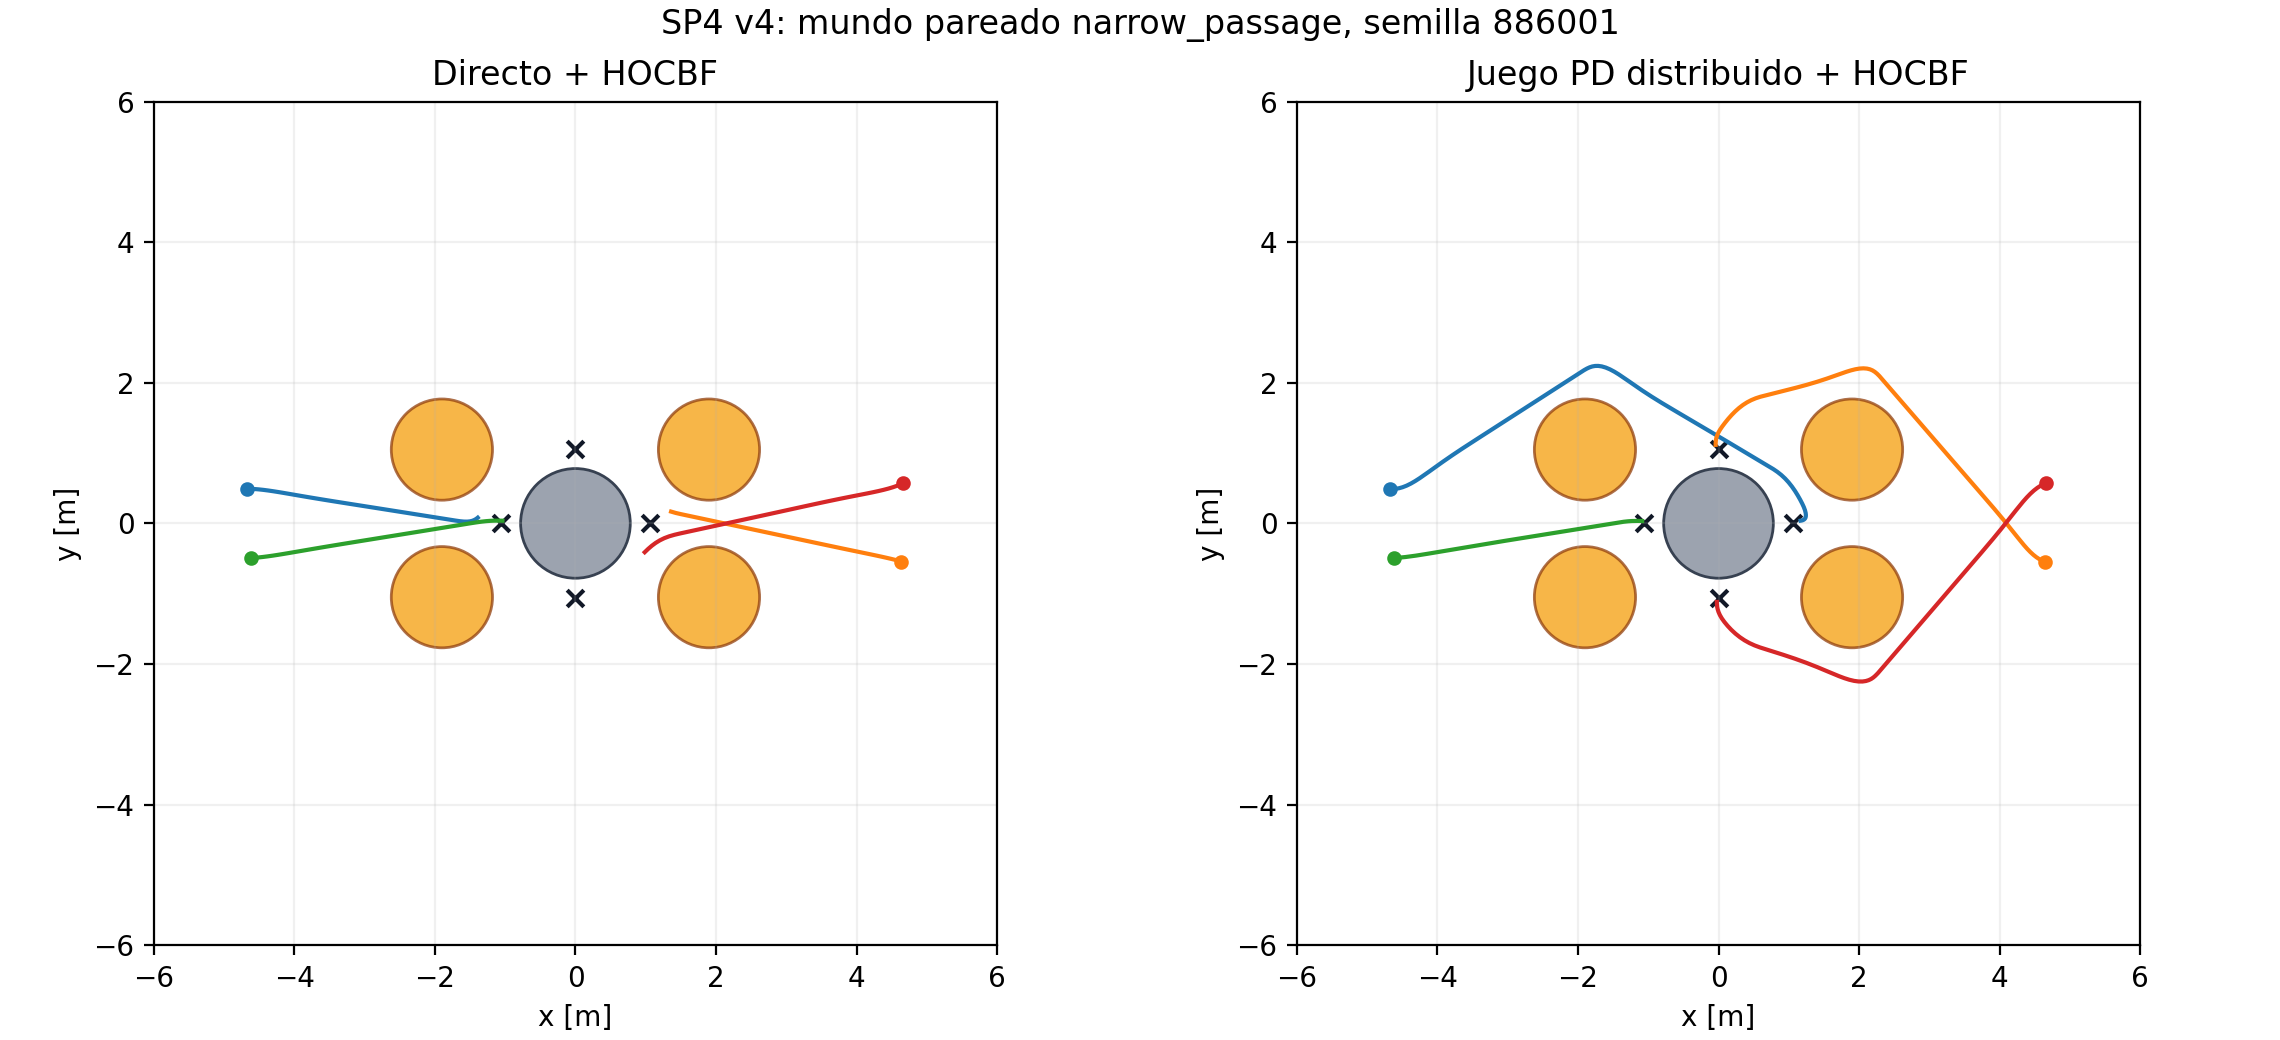
\includegraphics[width=0.92\textwidth]{figures/coppelia/sp4-v4-paired-trajectories.png}
  \caption[Trayectorias reproducidas en CoppeliaSim del mundo pareado de paso estrecho.]{Trayectorias
  reproducidas en CoppeliaSim del mundo pareado de paso estrecho. El método
  directo cruza las cuatro trayectorias dentro del cuello de botella; el juego
  PD distribuido con HOCBF las negocia y evita la colisión con el mismo
  origen, destino y semilla.}
  \label{fig:coppelia-narrow-trajectories}
  \viusource{elaboración propia, \texttt{run\_sp4\_v4\_coppelia\_paired\_scene.py}}
\end{figure}

La reproducción reproduce, en un motor distinto, el mismo desenlace cualitativo
que el modelo cinemático de E4; ser consistente con aquel resultado no es
confirmarlo, por las razones del párrafo anterior. Es una campaña separada del
piloto de almacén AWS de la Sección~\ref{sec:method_statistics_coppelia}, con
su propia escena y su propio protocolo de admisión, lo que la hace distinta de
aquella pero no una validación independiente de E4. El Anexo~\ref{app:sp2-coppelia-full-detail}
recoge esas comprobaciones, el vídeo y el CSV de poses medidas.

\zlabel{budget:coppelia-end}
